\documentclass[a4paper,12pt]{article}

\usepackage{rotating}
\usepackage[top=1in, bottom=1in, left=0.75in, right=0.75in]{geometry}
\usepackage{graphicx}
\usepackage[numbers,square,sort&compress]{natbib}
\usepackage{setspace}
\usepackage[cdot,mediumqspace,]{SIunits}
\usepackage{caption}
\usepackage{subcaption}
\usepackage{mathtools}
\usepackage{authblk}
\usepackage{float}
\renewcommand{\thesubsection}{\thesection.\alph{subsection}}
\providecommand{\e}[1]{\ensuremath{\times 10^{#1}}}

\begin{document}
\onehalfspacing
\title{PHY 407 Lab 6}
\author{Natalie Price-Jones, 999091021}
\date{17 October 2014}
\affil{\small{natalie.price.jones@mail.utoronto.ca}}
\maketitle

\section{Question 1}

\begin{figure}[H]
\centering
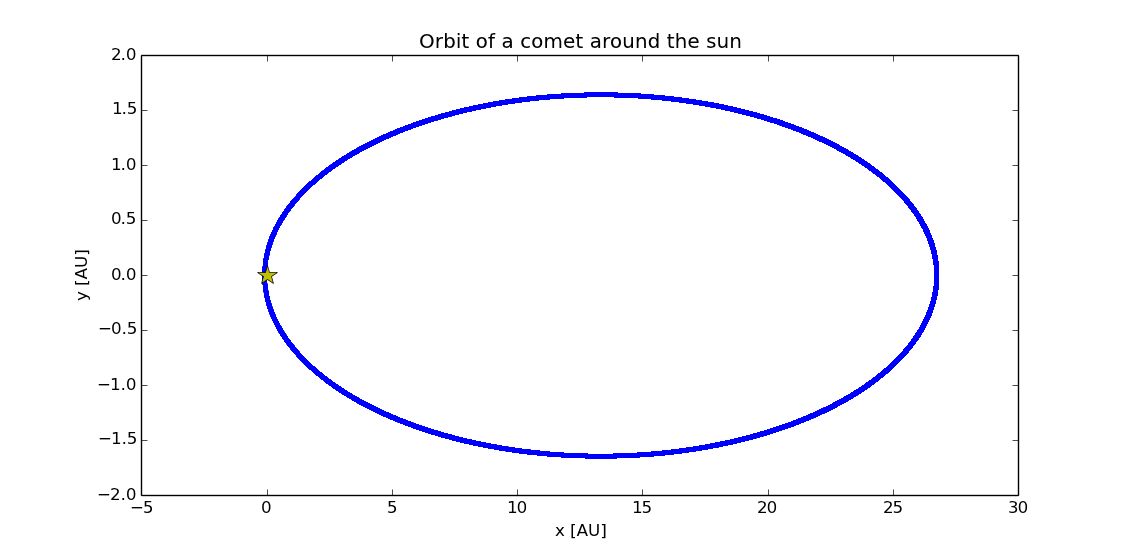
\includegraphics[width = \linewidth]{lab6q1.png}
\caption{Orbit integration with a fixed step size}
\label{fig:q1}
\end{figure}
 
Figure \ref{fig:q1} was made with a step size of 0.0005 years. The calculation took, on average, about 42 seconds to run.

\section{Question 2}

\begin{figure}[H]
\centering
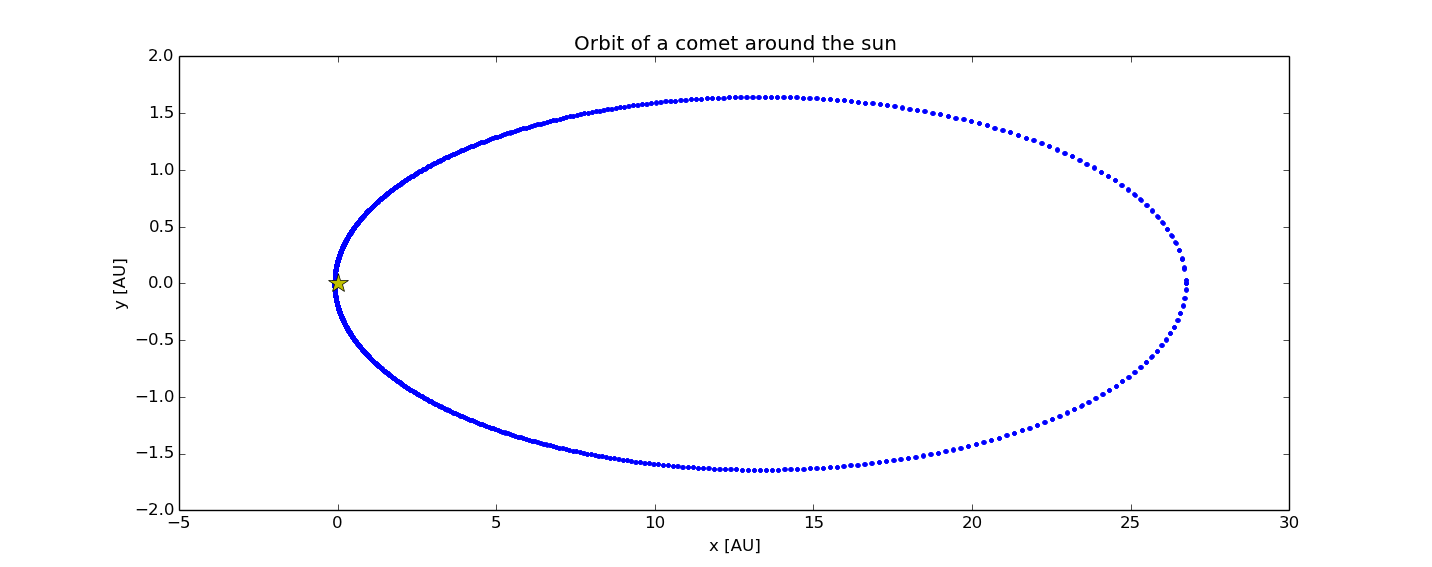
\includegraphics[width = \linewidth]{lab6q2.png}
\caption{Orbit integration with adaptive step size}
\label{fig:q2}
\end{figure}

Figure \ref{fig:q2} was made with varying step size, shown in Figure \ref{fig:q2i}. The calculation took, on average, 0.65 seconds to run. This is a vast improvement on the fixed step size method. The trade off came in the error, which on average was $3.8\e{-10} AU$, compared with $2.5\e{-12} AU$ in the previous part. This error could be adjusted, however, by chaning the $\delta$ parameter that determined the desired level of accuracy. If $\delta$ was changed from 1 km to 1 m, for example, runtime increased to about 5 seconds, but error was reduced to $6.0\e{-14} AU$.

\begin{figure}[H]
\centering
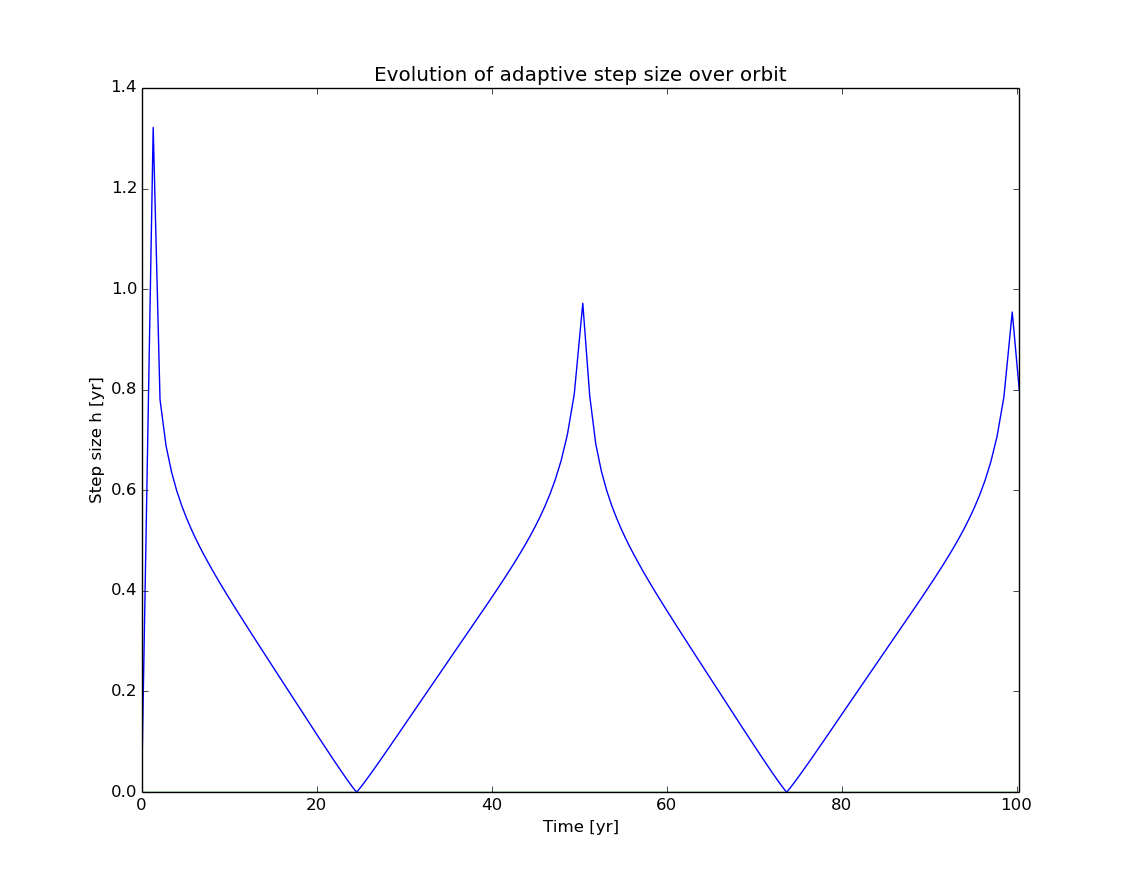
\includegraphics[width = \linewidth]{lab6q2additional.png}
\caption{Adaptive step size over time. As expected (barring some strange behviour in the first few integration steps due to apparently zero errors) the step size varies periodically as the orbit does. Also as expected, adaptive step size increases when the comet is far from the sun and decreases as it approaches. The fixed step size of h = 0.0005 is not even visible on the scale size of this plot, so adaptive methods obviously represent a vast improvement.}
\label{fig:q2i}
\end{figure}

\section{Question 3}

\begin{figure}[H]
\centering
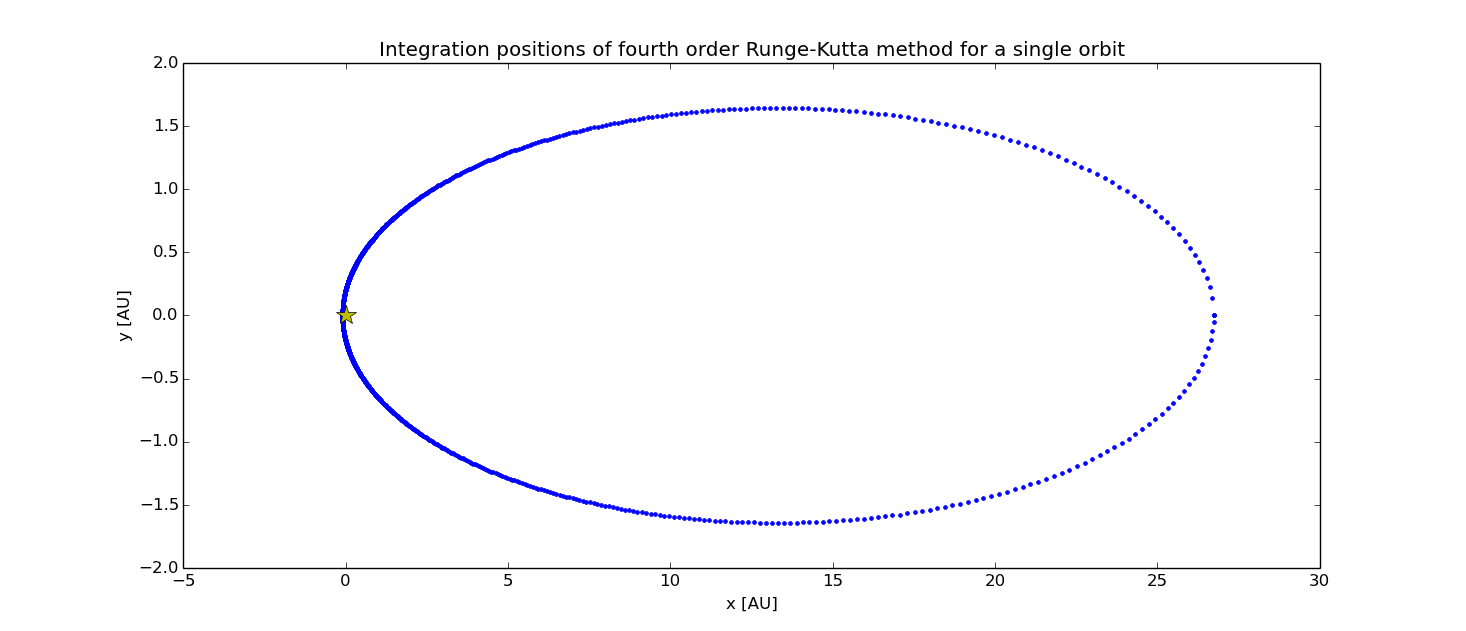
\includegraphics[width = \linewidth]{lab6q3.png}
\caption{}
\label{fig:q3}
\end{figure}

\section{Question 5}

For this part, I have included the plots of trajectories in position space as well as plotting both x and y trajectories against time. This was done to demonstrate motion that was not always obvious in the position space plots. All points have been colour coded to represent their position in time - red points are at early times and blue points are at late times. The position of the point on the timescale from 0 to 2 time units is indicated by its position in the rainbow spectrum between red and blue. 

\subsection{Part a)}
\begin{figure}[H]
\centering
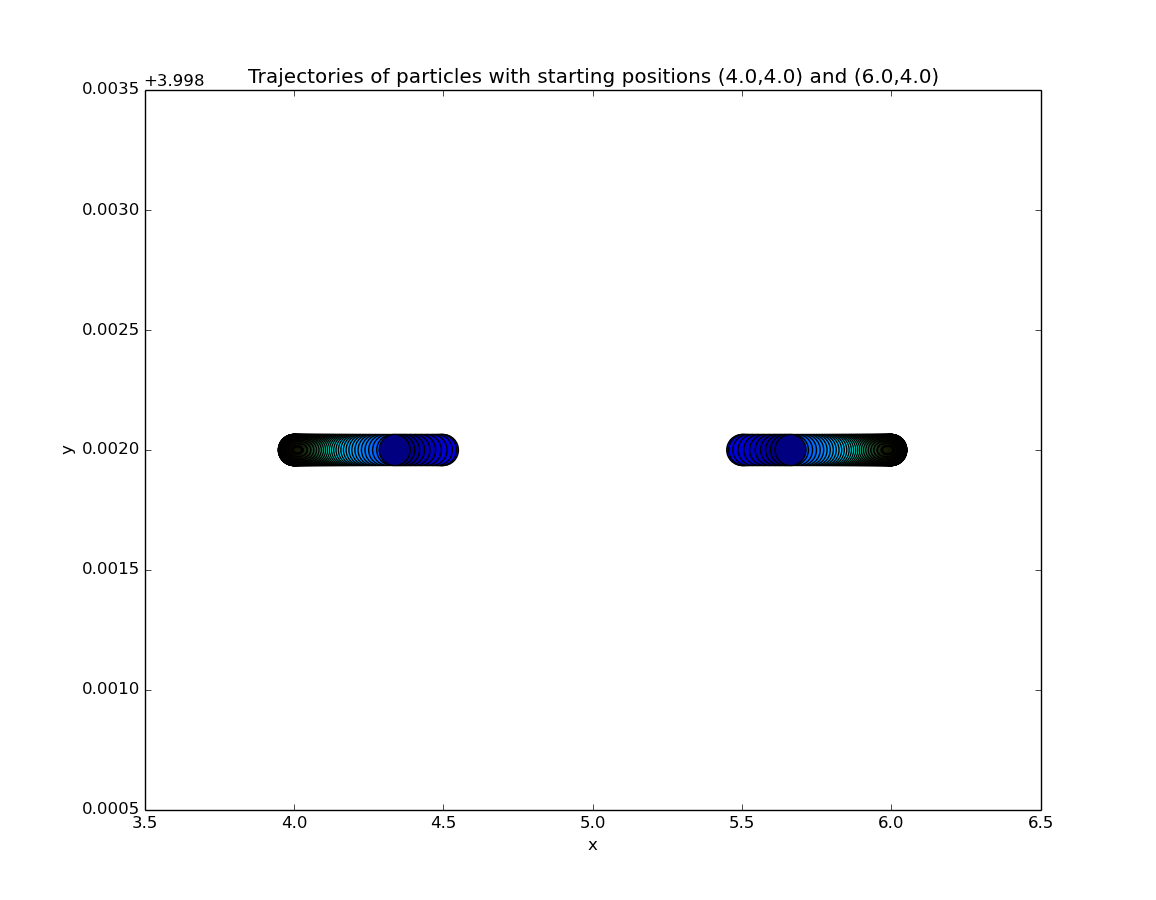
\includegraphics[width = \linewidth]{lab6q5a.png}
\caption{}
\label{fig:q5a}
\end{figure}

\begin{figure}[H]
\centering
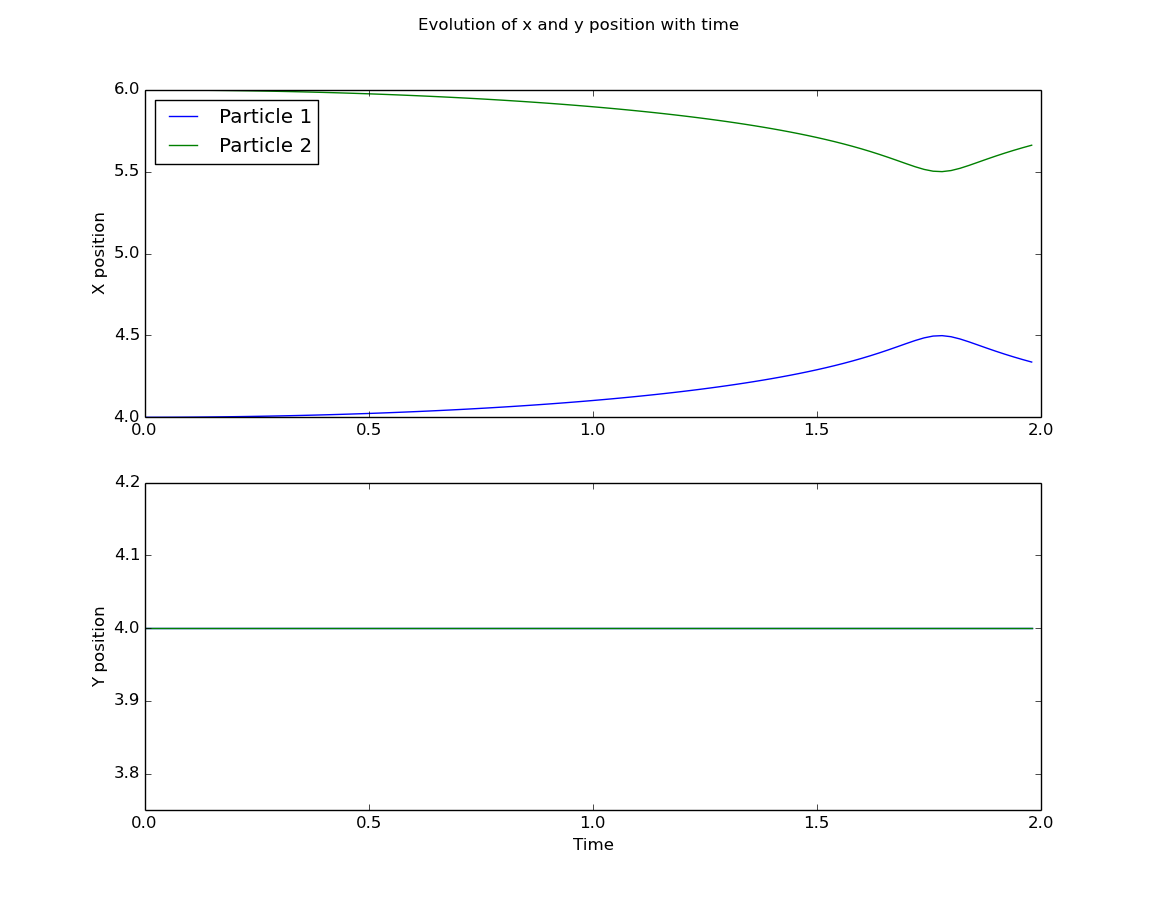
\includegraphics[width = \linewidth]{lab6q5ai.png}
\caption{As expected, there is no y-motion, since the particles lie along the same line in y. However, the behaviour in x is more dramatic. As expected, at larger separations, the particles attract each other, but as they grow closer they begin to repel.}
\label{fig:q5ai}
\end{figure}

\subsection{Part b)}

\begin{figure}[H]
\centering
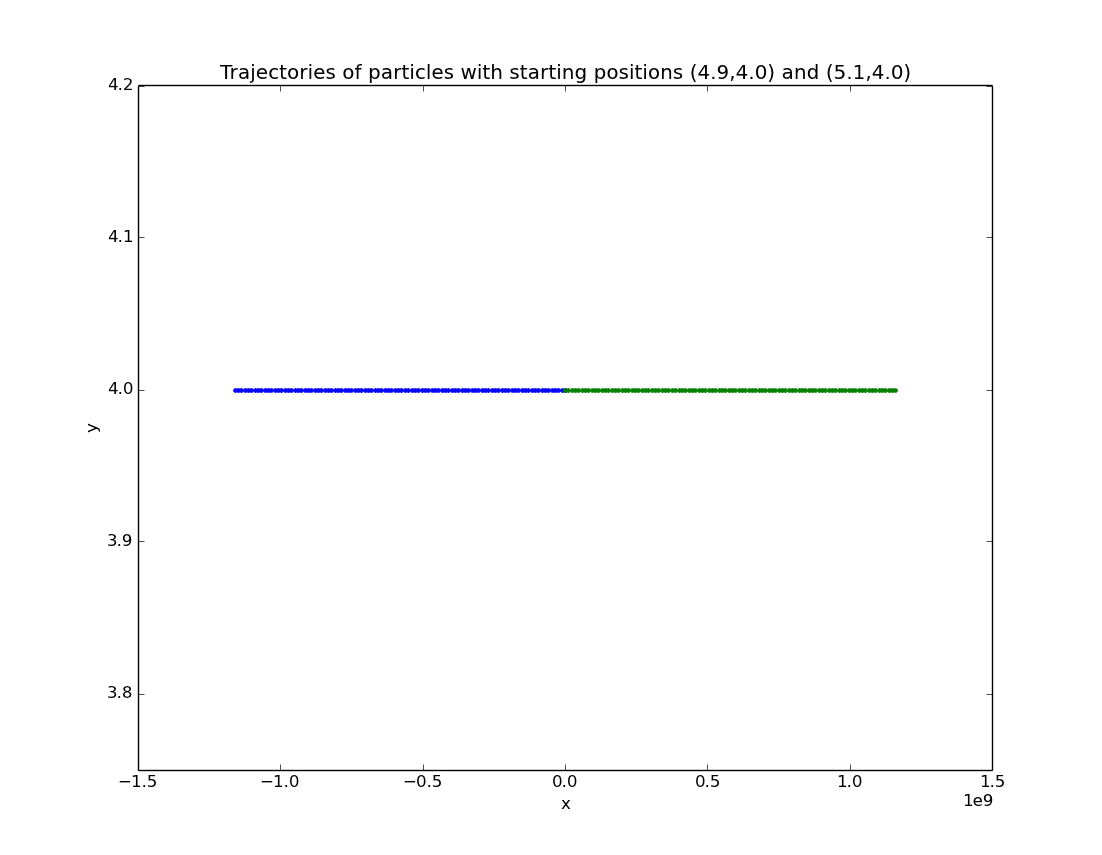
\includegraphics[width = \linewidth]{lab6q5b.png}
\caption{}
\label{fig:q5b}
\end{figure}

\begin{figure}[H]
\centering
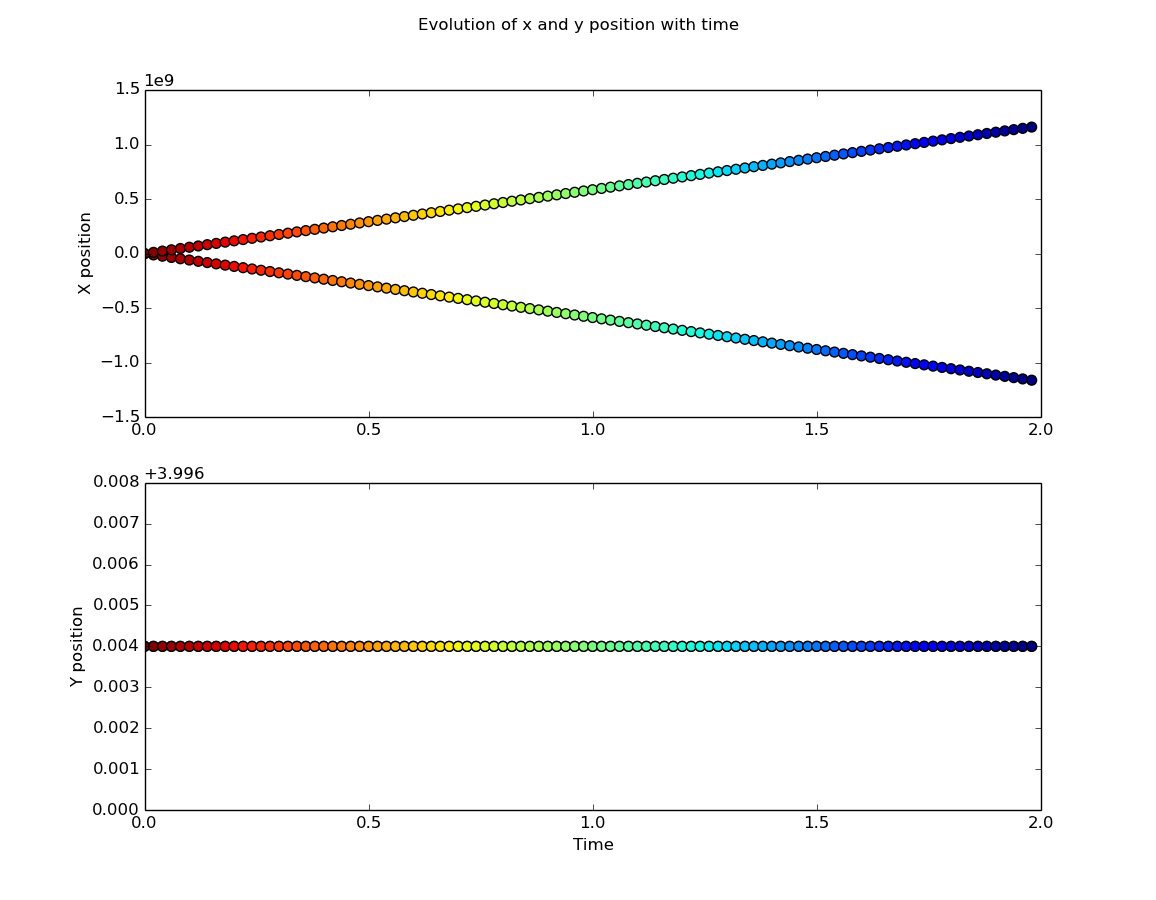
\includegraphics[width = \linewidth]{lab6q5bi.png}
\caption{In this case the particles begin so close together that the repulsive force generates a very strong acceleration away. Thus the two particles go off to $-\infty$ and $\infty$ respectively in x. The y direciton still sees no motion because both particles begin at constant y and there is no force to perturb them from it.}
\label{fig:q5bi}
\end{figure}

\subsection{Part c)}

\begin{figure}[H]
\centering
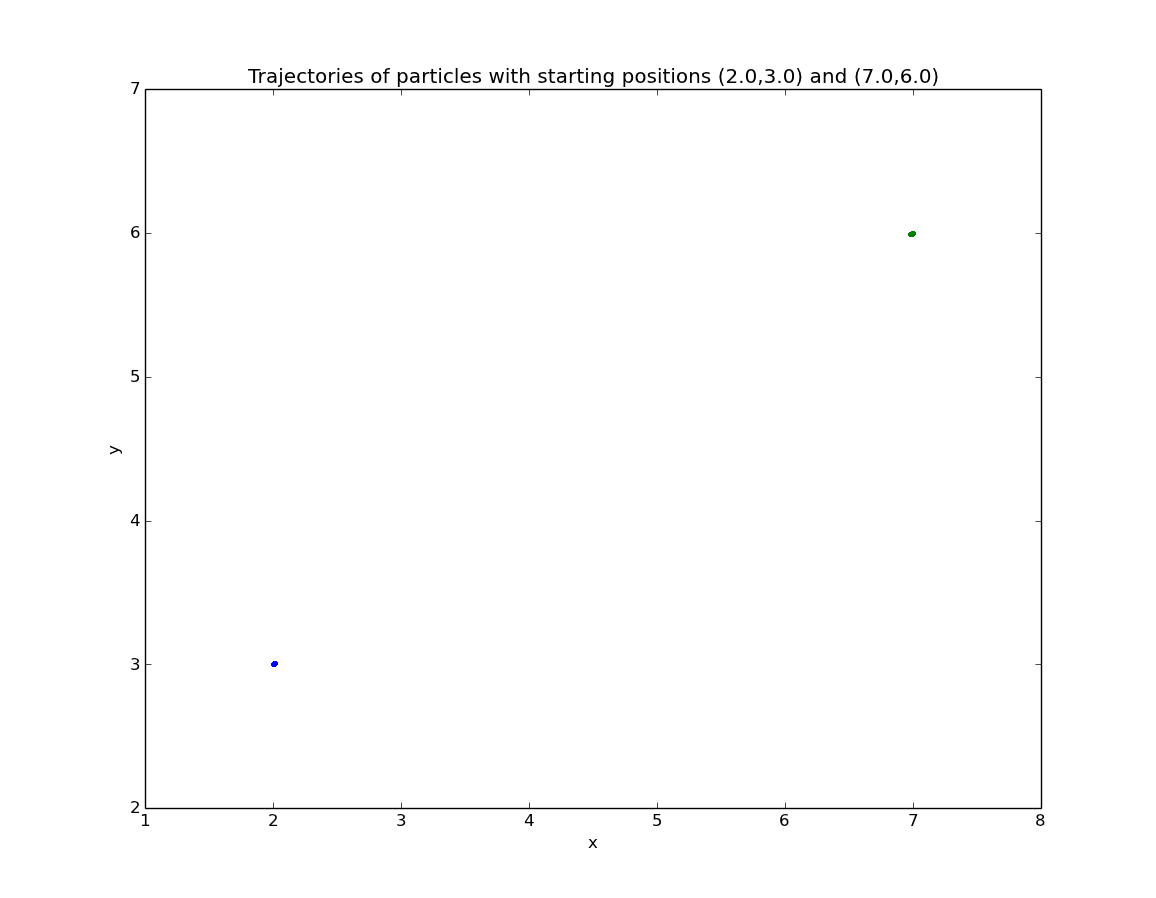
\includegraphics[width = \linewidth]{lab6q5c.png}
\caption{}
\label{fig:q5c}
\end{figure}

\begin{figure}[H]
\centering
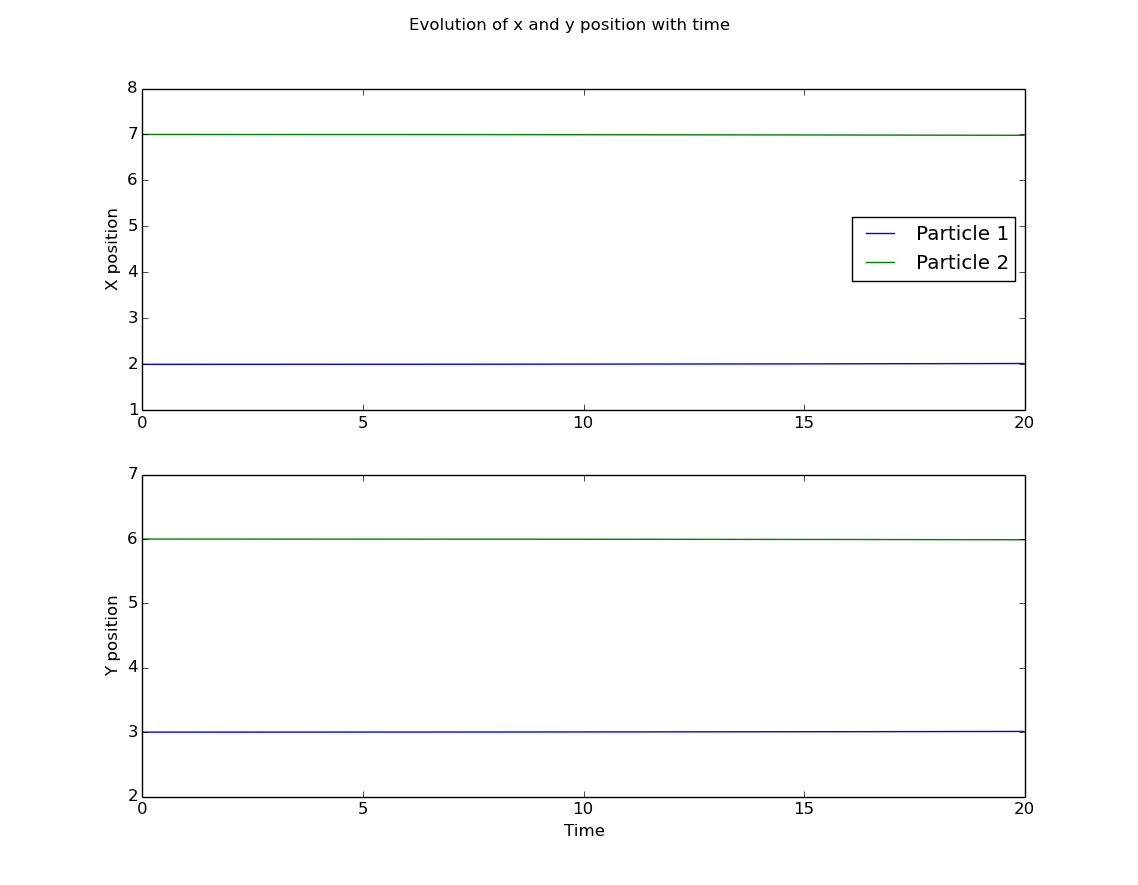
\includegraphics[width = \linewidth]{lab6q5ci.png}
\caption{These two particles started far enough apart that neither the attractive or repulsive forces are significant (or if they are, their components cancel), so the particles do not move from their initial position.}
\label{fig:q5ci}
\end{figure}

\subsection{Part d)}

\begin{figure}[H]
\centering
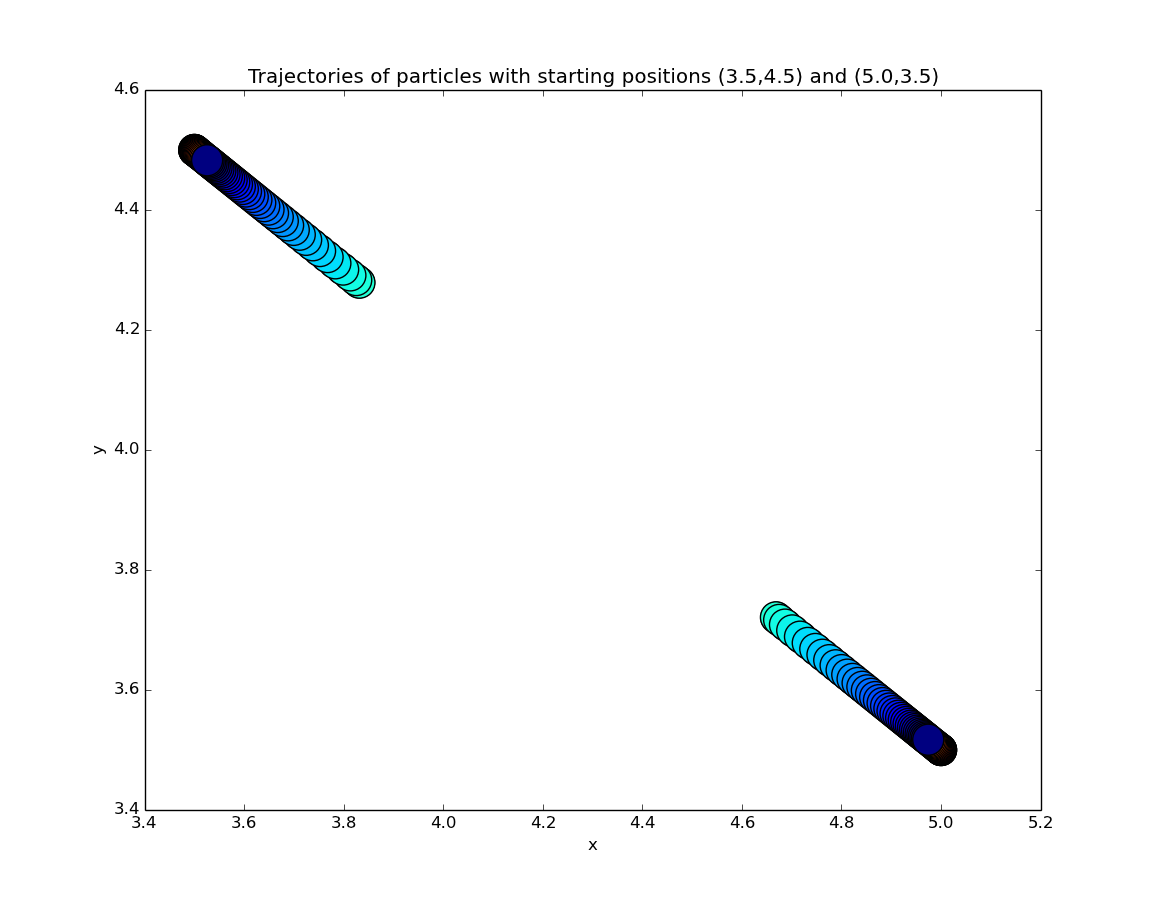
\includegraphics[width = \linewidth]{lab6q5d.png}
\caption{}
\label{fig:q5d}
\end{figure}

\begin{figure}[H]
\centering
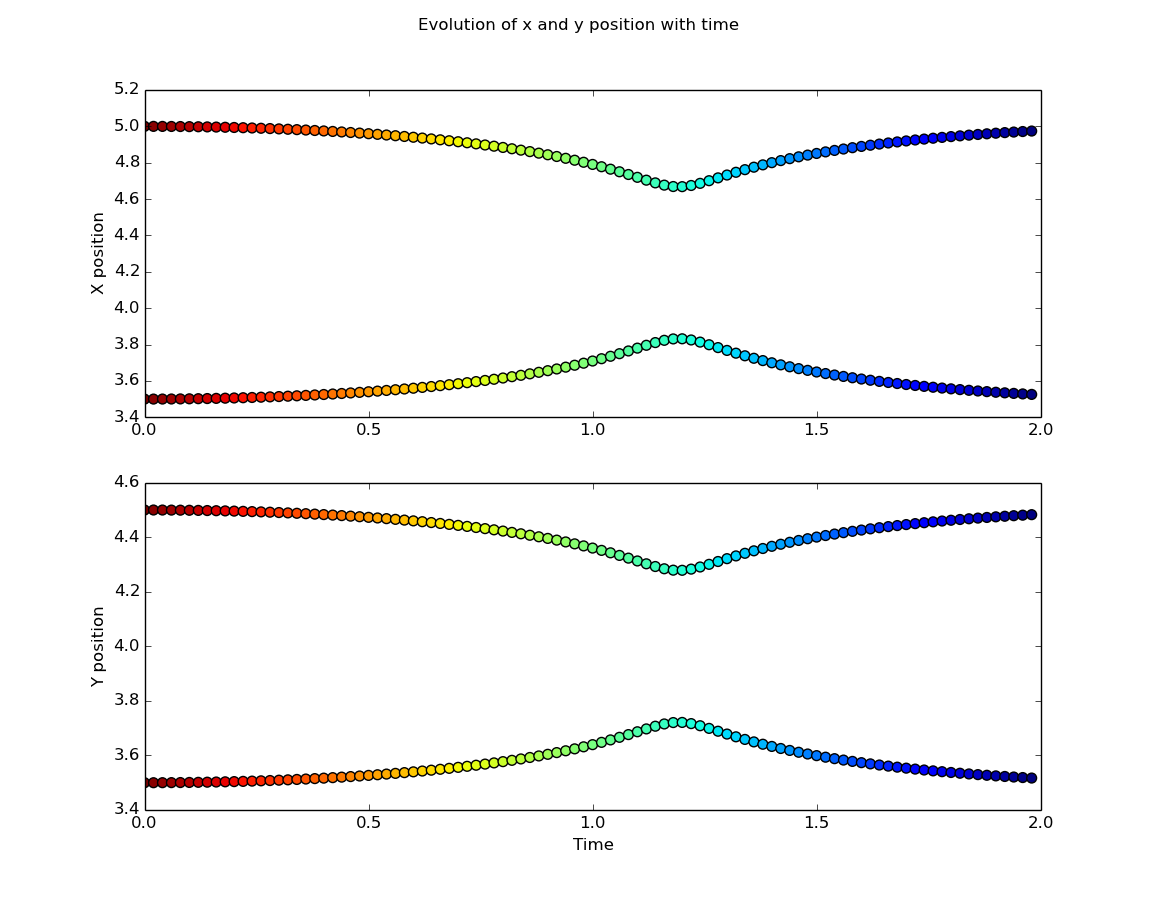
\includegraphics[width = \linewidth]{lab6q5di.png}
\caption{For these intial conditions, the two particles oscillate in both x and y, neither escaping each other's influence as in Figure ~\ref{fig:q5b} nor remaining inured to each other's presence as in Figure ~\ref{fig:q5c}. While only one cycle is shown here, extending integration time reveals that these particles are bound to oscillate this way for all time.}
\label{fig:q5di}
\end{figure}

\section{Question 6}

\begin{figure}[H]
\centering
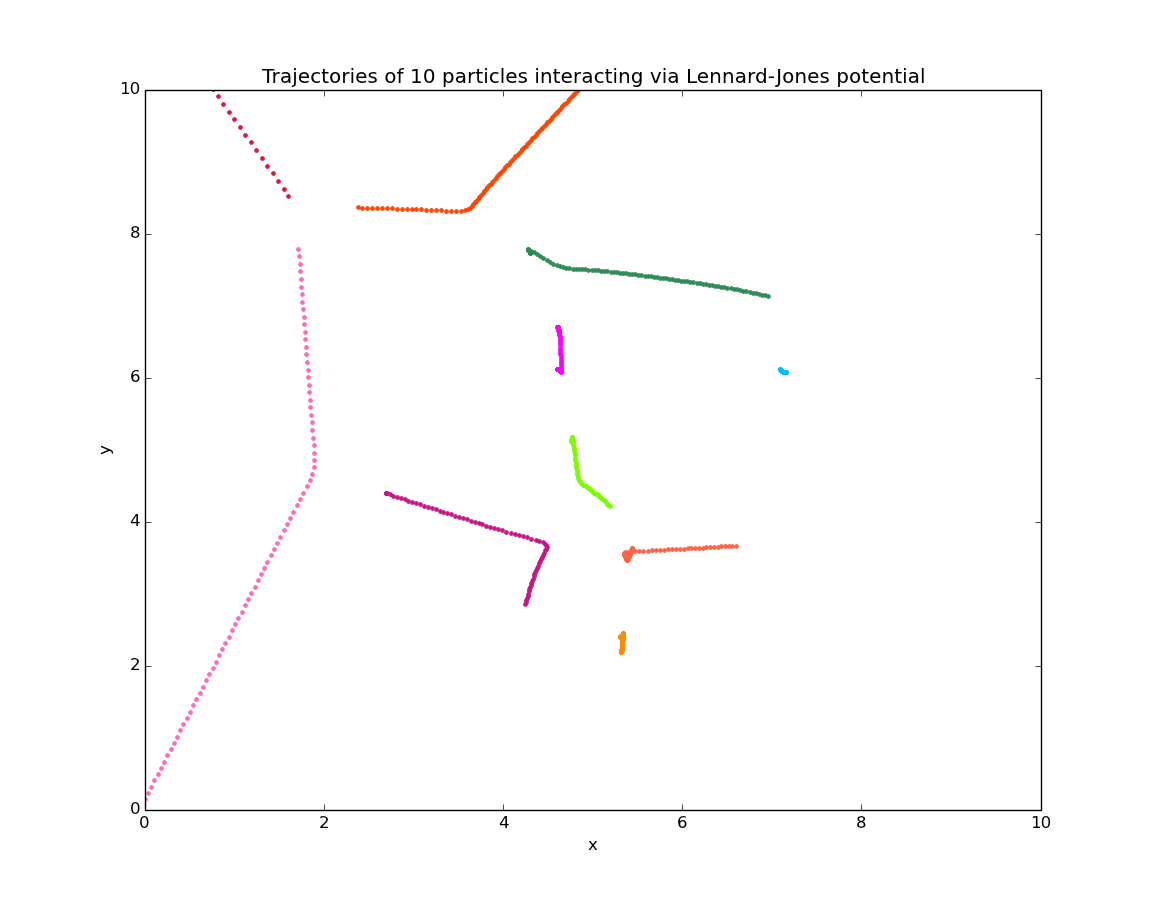
\includegraphics[width = \linewidth]{lab6q6_1.png}
\caption{}
\label{fig:q6}
\end{figure}

\section{Question 7}

\begin{figure}[H]
\centering
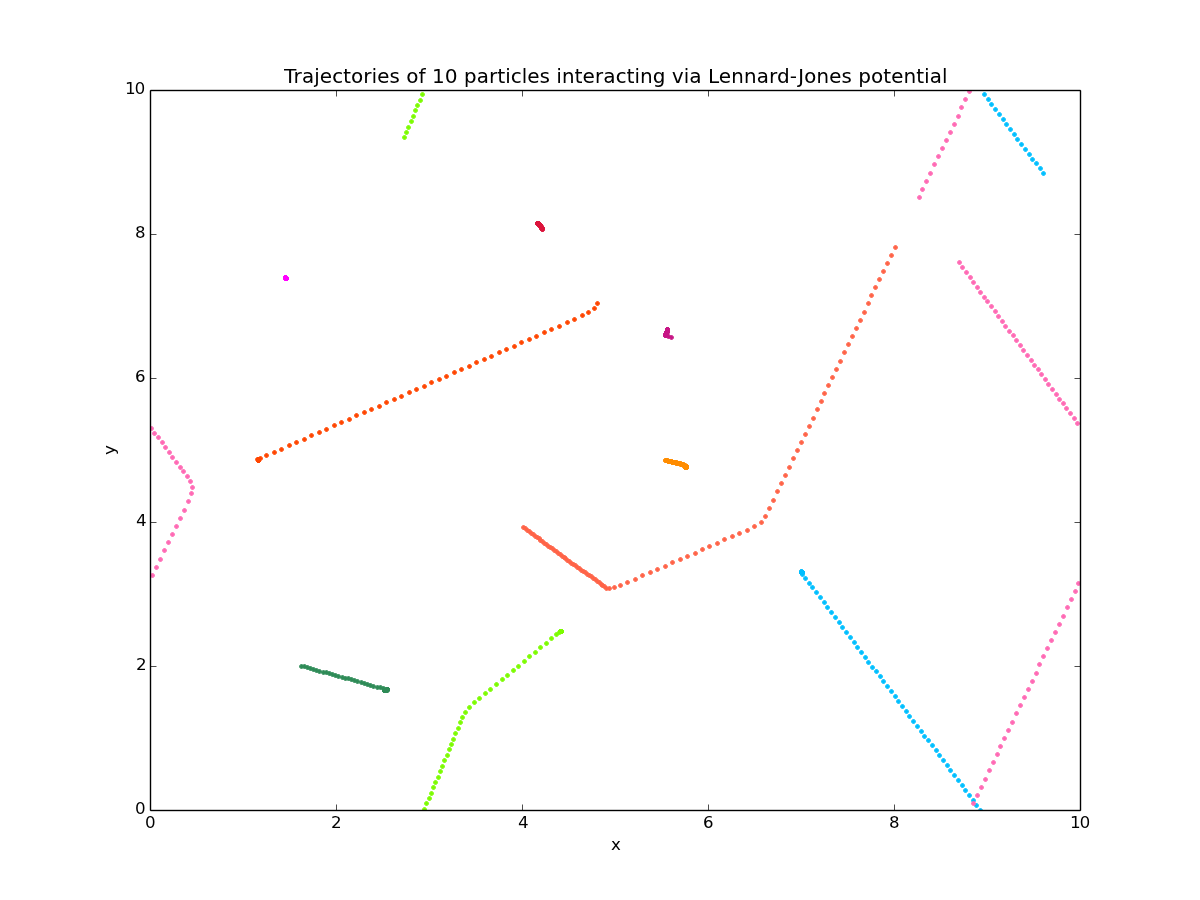
\includegraphics[width = \linewidth]{lab6q7_5.png}
\caption{}
\label{fig:q7}
\end{figure}

\section{Question 8}

\begin{figure}[H]
\centering
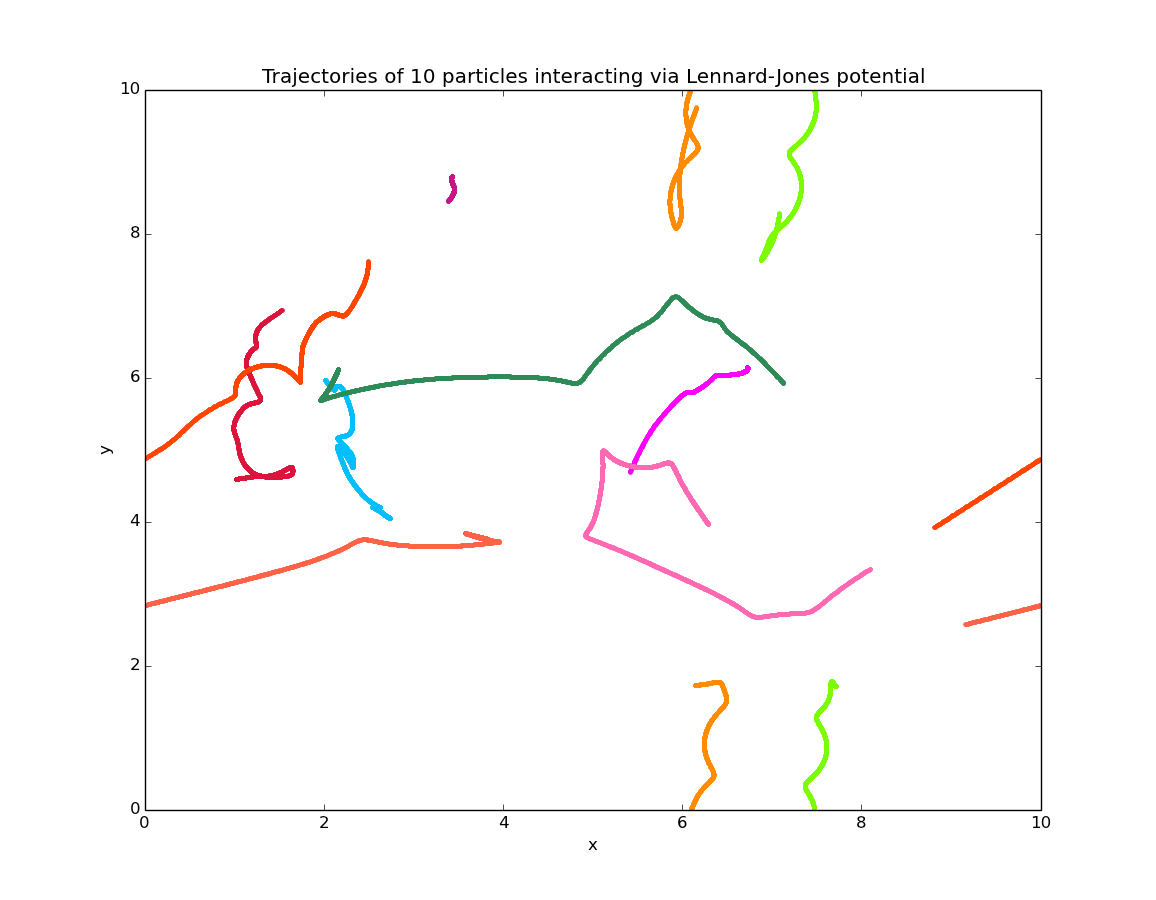
\includegraphics[width = \linewidth]{lab6q8.png}
\caption{}
\label{fig:q8}
\end{figure}

\end{document}





